\documentclass[12pt,a4paper]{article}  % шаблон для статьи, шрифт 12 пт
\usepackage[utf8x]{inputenc}  % использование кодировки Юникод UTF-8
\usepackage[russian]{babel}  % пакет поддержки русского языка
\usepackage{lipsum}  % Рыба-текст
\usepackage[compact]{titlesec}  % для titlespacing
\titlespacing*{\section}{0.75cm}{1em}{0.1em}  % отступ заголовка 
% \titlespacing{\заголовок}{слева}{перед}{после}[справа]
\titlespacing*{\subsection}{0.75cm}{1em}{0.1em}
\usepackage{indentfirst}  % отступ первого абзаца
\setlength{\parindent}{0.75cm}
\usepackage[labelsep=endash]{caption}  % тире вместо двоеточия в картинках
\usepackage{graphicx}  % кртинки
\usepackage{comment}  % комментарии
\usepackage{tabularx}  % таблицы
\usepackage{color}  % цветной код
\usepackage{listings}  % листинги кода из файлов
\usepackage{cite}  % ???
\lstset{ %
	language=C++,                   % выбор языка для подсветки (здесь это С++)
	basicstyle=\small,              % размер и начертание шрифта для подсветки кода
	numbers=left,                   % где поставить нумерацию строк (слева\справа)
	numberstyle=\tiny,              % размер шрифта для номеров строк
	stepnumber=1,                   % размер шага между двумя номерами строк
	numbersep=5pt,                  % как далеко отстоят номера строк от подсвечиваемого кода
	backgroundcolor=\color{white},  % цвет фона подсветки - используем \usepackage{color}
	showspaces=false,               % показывать или нет пробелы специальными отступами
	showstringspaces=false,         % показывать или нет пробелы в строках
	showtabs=false,                 % показывать или нет табуляцию в строках
	frame=false,                    % рисовать рамку вокруг кода
	tabsize=2,                      % размер табуляции по умолчанию равен 2 пробелам
	captionpos=t,                   % позиция заголовка вверху [t] или внизу [b] 
	breaklines=true,                % автоматически переносить строки (да\нет)
	breakatwhitespace=false,        % переносить строки только если есть пробел
	escapeinside={\%*}{*)}          % если нужно добавить комментарии в коде
}

%перенос строк внутри таблиц
\newcommand{\specialcell}[2][c]{%
	\begin{tabular}[#1]{@{}c@{}}#2\end{tabular}}

% нумерация рисунков по номеру главы (e.g. 1.1) для отчёта по курсовой
% \renewcommand\thefigure{\arabic{section}.\arabic{figure}}

% Шаблон создания картинки
% \begin{figure}[hpt!]
% 	\centering
% 	\includegraphics[width=0.6\linewidth]{photo/photo1}
% 	\caption{Подпись к рисунку}
% 	\label{имя ссылки на рисунок}
% \end{figure}

\begin{document}
	
	\thispagestyle{empty}
	
	\begin{center}
		\Large{
			\textbf{МИНОБРНАУКИ РОССИИ}
			
			\textbf{Санкт-Петербургский государственный}
			
			\textbf{электротехнический университет «ЛЭТИ»}
			
			\textbf{им. В.И. Ульянова (Ленина)}
			
			\textbf{Кафедра САПР}
		}
	\end{center}
	
	\topskip=0pt
	\vspace*{\fill}
	\begin{center}
		\Large{
			\textbf{
				ЛАБОРАТОРНАЯ РАБОТА №1\\
				по дисциплине «Программирование»\\
				Тема: Массивы указателей. Динамическое
				управление памятью\\
			}
		}
	\end{center}
	\vspace*{\fill}
	
	\begin{tabular}{lcr}
		Студенты гр. 9892 & \begin{tabular}{p{60mm}} \\ \hline \end{tabular} & Лескин К.А.  \\\\
		& \begin{tabular}{p{60mm}} \\ \hline \end{tabular} & Миллер В.В. 
		\\\\
		Преподаватель    & \begin{tabular}{p{60mm}} \\ \hline \end{tabular} & Кузьмин С.А. 
		\\\\
	\end{tabular} 
	
	\begin{center}
		Санкт-Петербург\\
		2020
	\end{center}
	%////////////////////////////////////////////////////////////////////////////////////////////////
	%////////////////////////////////////////////////////////////////////////////////////////////////
	%////////////////////////////////////////////////////////////////////////////////////////////////
	\newpage
	
	\section*{Цель работы}
	
	Получение
	практических
	навыков
	разработки
	программы,
	обрабатывающей данные, представленные массивом указателей.
	
	\section*{Формулировка задания}
	
	Разработать программу, обрабатывающую текстовую информацию,
	представленную массивом указателей на строки (массивы символов).
	Программа должна считать данные (текстовую информацию) из
	входного файла, представленного набором строк (каждая строка
	представляет собой последовательность символов, среди которых могут быть
	буквы, пробелы, знаки препинания и т.п.). 
	
	Далее над текстом выполняется
	операция, определённая в вариантах задания. После чего результаты
	выполнения операции должны быть отражены на экране и записаны в новый
	файл.
	
	Доступ к каждой строке массива, а также к отдельному элементу
	(символу) строки должно осуществляться через указатели.
	
	Индивидуальный вариант: Удалить все слова, содержащие заданный символ, в каждой строке текста.
	
	\section*{Форматы входных и выходных файлов}
	
	Входной файл может иметь любую структуру, главное, чтобы он был текстовым.
	
	Выходной файл запысывается следующем формате:
	\begin{itemize}
		\item вначале должны быть записаны исходные строки;
		\item потом должно быть записано название совершённой операции;
		\item потом должны быть записаны введённые данные и параметры;
		\item после чего уже должны быть записаны полученные строки.
	\end{itemize}
	
	\newpage
	\section*{Описание структур данных}
	
	Для хранения строк, считанных из файла, используется массив указателей на строки. Доступ к массиву осуществляется через указатель на него. Память под строки и массив указателей на них выделяется динамически. Структура хранения данных указана на рис. \ref{data_schema}.
	\begin{figure}[hpt!]
		\centering
	 	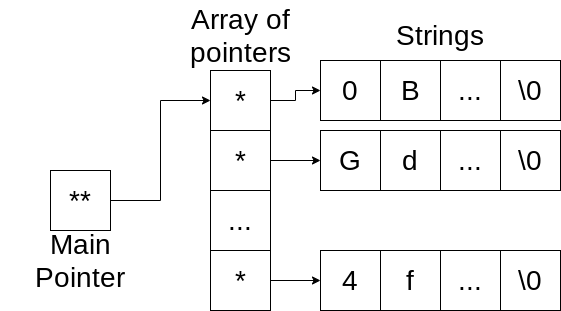
\includegraphics[width=0.6\linewidth]{photo/data_schema}
	 	\caption{Структура хранения данных, считанных из файла}
	 	\label{data_schema}
	\end{figure}
	
	\section*{Описание пользовательских функций}
	
	\subsection*{DeleteWordsWithChar}
	void DeleteWordsWithChar(char *strings[], int lines\_number, char bad\_char);
	
	Функция по удалению слов, содержащих заданный символ, из массива строк. Принимает указатель на массив строк, количество строк и символ, который должен содержаться в словах для удаления.
	
	\if 0
	
	Алгоритм работы функции:
	
	Цикл по line от 0 до lines\_number
		\begin{itemize}
			\item Записываем указатель на текущую строку в string
			\item Выделяем память под новую строку и записываем указатель в new\_string
			\item Выделяем память под слово и записываем указатель в word
			\item Если IfStringContainsChar для текущей строки возвращает \textbf{false}, сбрасываем текущую итерацию цикла
			\item Цикл по character\_pos от 0 до длины string
			\begin{itemize}
				\item Записываем текущий символ в character
				\item Если character == ' ' или character == '\textbackslash n' или character == EOF или character == '\textbackslash 0'
				\begin{itemize}
					\item Если IfStringContainsChar возвращает \textbf{true} для word
					\subitem strcat(new\_string, word)
					\subitem strcat(new\_string, character)
					\item Освободить указатель word
					\item Выделить память под слово и записать указатель в word
					\item Сбросить текущую итерацию цикла
				\end{itemize}
				\item Иначе
				\subitem strcat(word, character);
			\end{itemize}
		\item Освобождаем указатель на проверенную строку
		\item Если послений символ строки не \textbackslash n, добавляем \textbackslash n в конец
		\item Присваиваем указателю адрес ячейки памяти, на которую указывает new\_string
		\end{itemize}
	
	\fi
	
	\subsection*{ReadFromFile}
	int ReadFromFile(const std::string\& file\_name, char **\&strings);
	
	Функция для чтения строк из файла. 
	
	Принимает имя файла и ссылку на указатель на указатель на char (необходимо, чтобы модифицировать оригинальный указатель). 
	
	Возвращает количество прочитанных строк.
	
	\if 0
	
	Алгоритм работы функции:
	
	\begin{itemize}
		\item Пытемся открыть файл. В случаем провала возвращаем -1
		\item Задаём константы string\_chunk\_len = 10, lines\_chunk\_len = 3
		\item Выделяем память под массив строк длинной lines\_chunk\_len
		\item Выделяем память под нулевую строку длинной string\_chunk\_len
		\item Создаём место под считываемый символ
		\item Пока считанный из файла символ в current\_char не равен EOF
		\begin{itemize}
			\item ++line\_size
			\item Если длина строки line\_size кратна string\_chunk\_len, расширяем текущую строку на string\_chunk\_len
			\item Записываем считанный символ в текущую строку.
			\item Если считанный символ == \textbackslash n
			\begin{itemize}
				\item Записываем символ конца строки в текущую строку
				\item line\_size = 0
				\item ++line
				\item Если размер массива line кратен lines\_chunk\_len, расширяем массив строк на lines\_chunk\_len
				\item Выделяем память под нулевую строку длинной string\_chunk\_len
			\end{itemize}
		\end{itemize}
		\item Закрываем файл
		\item Возвращаем количество считанных строк
	\end{itemize}
	
	\fi
	
	\subsection*{WriteInFile}
	void WriteInFile(const std::string\&, char **, char **, char, int);
	
	Функция для записи массива строк в файл.
	
	Принимает указатель на массив оригинальных строк, указатель на массив изменённых строк, символ, который содержался в удалённых словах и количество строк.
	
	\if 0
	
	Алгоритм работы функции:
	
	\begin{itemize}
		\item Пытемся открыть файл. В случаем провала возвращаемся
		\item Записываем в файл оригинальные строки
		\item Записываем в файл совершённую операцию
		\item Записываем в файл параметры операции
		\item Записываем в файл модифицированные строки
		\item Закрываем файл
	\end{itemize}
	
	\fi
	
	\subsection*{IfStringContainsChar}
	bool IfStringContainsChar(char* string, char bad\_char);
	
	Функция для проверки содержания в строке заданного символа.
	
	Принимает указатель на строку и проверяемый символ.
	
	Возвращает true, если символ найден, false в противном случае.
	
	\if 0
	
	Алгоритм работы функции:
	
	\begin{itemize}
		\item Записываем указатель на строку в word\_ptr
		\item Пока значение word\_ptr не 0
		\begin{itemize}
			\item Если strchr(\&bad\_char, *word\_ptr) Возвращаем \textbf{true}
			\item ++word\_ptr
		\end{itemize}
		\item Возвращаем \textbf{false}
	\end{itemize}
	
	\fi
	
	\subsection*{PrintArrayOfStrings}
	void PrintArrayOfStrings(char **strings, int lines\_number);
	
	Функция для печати массива строк.
	
	Принимает указатель на массив строк и количество строк.
	
	\if 0
	
	Алгоритм работы функции:
	
	\begin{itemize}
		\item Циклом по line от 0 до lines\_number печатаем строку
	\end{itemize}
	
	\fi
	
	\subsection*{strcat}
	char *strcat (char *dest, char character);
	
	Перегрузка функции strcat из strings.h. 
	
	Принимает указатель на исходную строку и символ для добавления в конец.
	
	Возвращает указатель на новую строку с добавленным символом.
	
	\if 0
	
	Алгоритм работы функции:
	
	\begin{itemize}
		\item Выделяем память под 2 символа (char\_ptr)
		\item В первую ячейку записываем character
		\item Во вторую ячейку записываем \textbackslash 0
		\item strcat(dest, char\_ptr)
		\item Освобождаем память char\_ptr
		\item Возвращаем указатель на dest
	\end{itemize}
	
	\fi
	
	\section*{Алгоритм программы}
	
	\begin{itemize}
		\item Вызываем ReadFromFile
		\item Проверяем, что файл считан успешно
		\item Переписываем считанные данные в original\_strings
		\item Считываем с клавиатуры символ
		\item Вызываем DeleteWordsWithChar
		\item Печатаем результат с помощью PrintArrayOfStrings
		\item Записываем Изменения в файл с помощью WriteInFile
	\end{itemize}
	
	\section*{Тестирование программы}
	
	Тесты с описанием действий. Обязательно картинки с результатами
	
	\section*{Выводы}
	
	Вывод
	
	\newpage
	\section*{Приложение А. Листинг программного кода}

	\subsection*{main.cpp}
	\lstinputlisting{src/main.cpp}
	
	\newpage
	\subsection*{delete\_words\_with\_char.cpp}
	\lstinputlisting{src/delete_words_with_char.cpp}
	
	\newpage
	\subsection*{delete\_words\_with\_char.h}
	\lstinputlisting{src/delete_words_with_char.h}
	
	\newpage
	\subsection*{files\_lib.cpp}
	\lstinputlisting{src/files_lib.cpp}
	
	\newpage
	\subsection*{files\_lib.h}
	\lstinputlisting{src/files_lib.h}
	
	\newpage
	\subsection*{if\_string\_contains\_char.cpp}
	\lstinputlisting{src/if_string_contains_char.cpp}
	
	\newpage
	\subsection*{if\_string\_contains\_char.h}
	\lstinputlisting{src/if_string_contains_char.h}
	
	\newpage
	\subsection*{print\_array\_of\_strings.cpp}
	\lstinputlisting{src/print_array_of_strings.cpp}
	
	\newpage
	\subsection*{print\_array\_of\_strings.h}
	\lstinputlisting{src/print_array_of_strings.h}
	
	\newpage
	\subsection*{strcat\_impl.cpp}
	\lstinputlisting{src/strcat_impl.cpp}
	
	\newpage
	\subsection*{strcat\_impl.h}
	\lstinputlisting{src/strcat_impl.h}
	
\end{document}